\documentclass[11pt,a4paper,landscape]{ctexart}

\usepackage[top=1.5cm,bottom=1.5cm,left=1.6cm,right=1.6cm]{geometry}
\usepackage{amsmath,amssymb}
\usepackage{graphicx}
\usepackage{booktabs}
\usepackage{multirow}
\usepackage{array}
\usepackage{float}
\usepackage{xcolor}
\usepackage{colortbl}
\usepackage{enumitem}
\usepackage{tikz}
\usepackage{hyperref}
\hypersetup{hidelinks}

\graphicspath{{figures/}}

\pagestyle{empty}

% —— 每页统一样式 ——
\newcommand{\slidetitle}[2]{%
    \noindent{\Large\bfseries #1}\hfill{\normalsize\color{gray!70!black} #2}\par
    \vspace{0.2em}
    \noindent\textcolor{gray!50}{\rule{\linewidth}{0.6pt}}\par
    \vspace{0.6em}
}

\newcommand{\footerline}{%
    \vfill
    \noindent\textcolor{gray!50}{\rule{\linewidth}{0.3pt}}\par
    \vspace{0.1em}
    {\footnotesize\color{gray!70} 数据截止 2026-07-09 10:54 \hfill EST-D-26-05697 项目情况报告 \hfill 陈清洋}
}

\begin{document}

%======================================================================
% 封面
%======================================================================
\begin{center}
\vspace*{2.2cm}
{\Huge\bfseries EST-D-26-05697 项目情况报告}\\[0.9em]
{\Large 拒稿后 4 周实验数据陈述}\\[3em]

\begin{tabular}{@{}rl@{}}
{\Large 报告类型}\quad & {\Large 内部报告，仅陈述事实} \\[0.6em]
{\Large 时间窗口}\quad & {\Large 2026-06-13 至 2026-07-09} \\[0.6em]
{\Large 数据规模}\quad & {\Large 35{,}100 数据点，5 数据集，17 方法} \\[0.6em]
{\Large 报告人}\quad & {\Large 陈清洋} \\
\end{tabular}

\vspace{3em}
\begin{tabular}{@{}p{18cm}@{}}
\centering\normalsize\itshape 本报告以图表为主，每页一个独立主题。判断留给读者。
\end{tabular}
\end{center}

\newpage

%======================================================================
% Page 1: 目录 / 讲什么
%======================================================================
\slidetitle{目录}{6 个独立主题}

\vspace{2em}
\begin{center}
\begin{tabular}{@{}rp{18cm}@{}}
\Large\textbf{01.} & \Large 原稿方法在文献时间线上的位置 \\[1em]
\Large\textbf{02.} & \Large 原稿 46--55\% MIM 提升的来源拆解 \\[1em]
\Large\textbf{03.} & \Large 4 周内完成的实验数据资产 \\[1em]
\Large\textbf{04.} & \Large 4 周内尝试过的三条新方法路径 \\[1em]
\Large\textbf{05.} & \Large 端到端方法 vs 两阶段插补的完整对比 \\[1em]
\Large\textbf{06.} & \Large GraphMIM 在跨数据集上的排名分布 \\
\end{tabular}
\end{center}

\footerline
\newpage

%======================================================================
% Page 2: 文献溯源
%======================================================================
\slidetitle{01 \quad 原稿方法在文献时间线上的位置}{R2 \#1 novelty 批评的事实依据}

\begin{table}[H]
\centering
\begin{tabular}{@{}p{4.5cm}p{9.5cm}p{9.5cm}@{}}
\toprule
\textbf{原稿方法} & \textbf{tex 中的实际操作} & \textbf{文献先例} \\
\midrule
缺失指示器 MIM \newline (§3.4, 算法 1) &
$m_{ij}=\mathbf{1}(x_{ij}\text{ missing})$，均值插补后拼接\newline$[\hat{X}|M]\in\mathbb{R}^{n\times 32}$ &
Jones 1996（统计学首创）\newline
Che 2018 GRU-D（引入深度学习 + 时间衰减）\newline
原稿去掉了 Che 的时间衰减和专用 GRU-D 结构 \\
\midrule
多缺失率联合训练 \newline (§4.3, 算法 2) &
将训练集在 $r\in\{0.0,0.1,\ldots,0.9\}$ 下\newline 生成 10 副本合并，扩大 10 倍 &
Srivastava 2014 输入 dropout\newline
Du 2023 SAITS mask-and-reconstruct 训练 \\
\bottomrule
\end{tabular}
\end{table}

\vspace{1.2em}
\begin{center}
\textbf{R2 \#1 原文批评：}
\end{center}

\begin{quotation}
\noindent\itshape "The core idea, concatenating imputed features with a binary missing indicator matrix as model input, is directly adopted from previous work in other domains (e.g., Che et al., 2018 for medical time series). The authors offer no methodological improvement or domain-specific adaptation tailored to battery systems."
\end{quotation}

\footerline
\newpage

%======================================================================
% Page 3: 46-55% 拆解
%======================================================================
\slidetitle{02 \quad 原稿 46--55\% MIM 提升的来源拆解}{R1 \#4 消融基线建议触及的证据结构}

\begin{minipage}[t]{0.58\textwidth}
\vspace{0.5em}
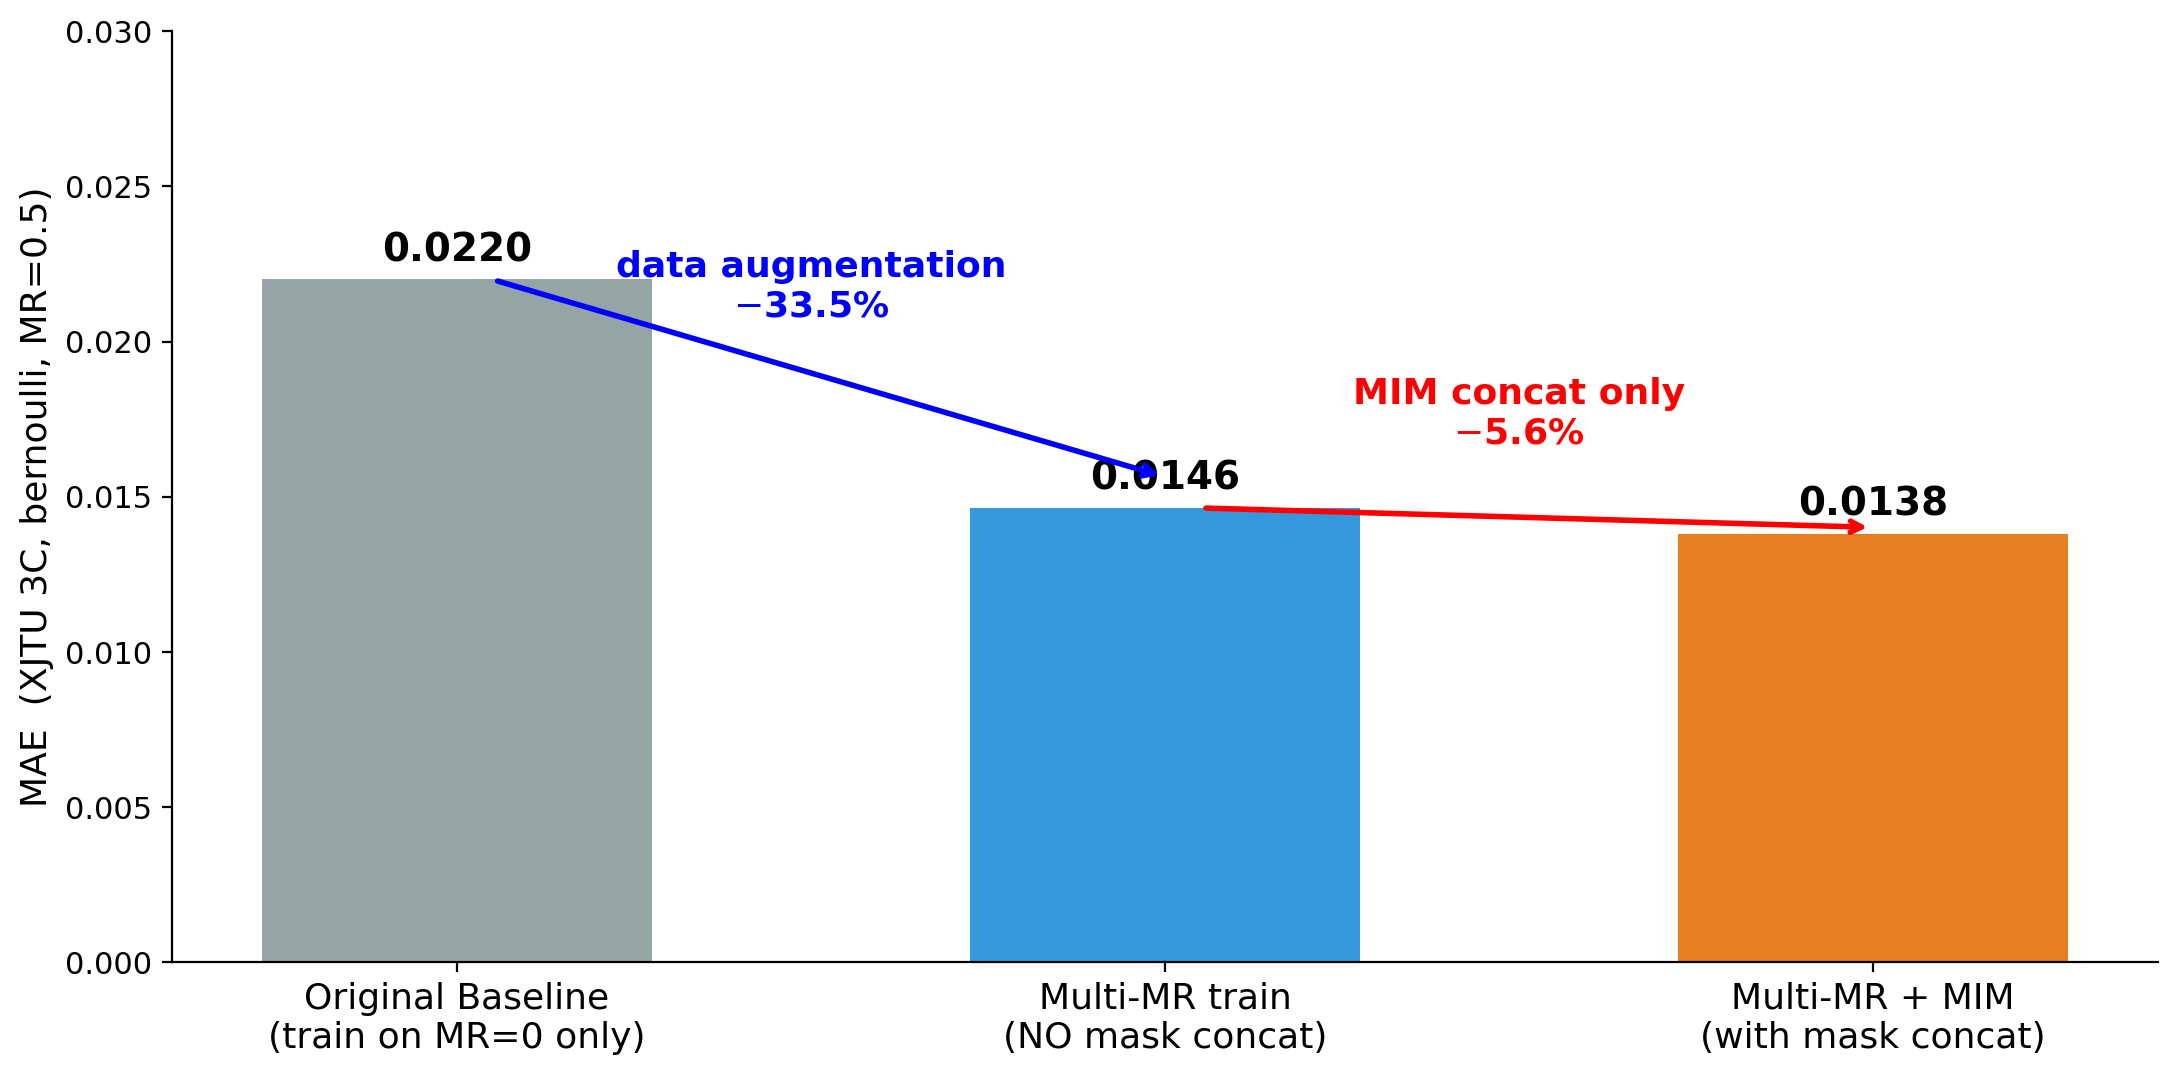
\includegraphics[width=\textwidth]{mim_effect_decomposition.png}
\end{minipage}\hfill
\begin{minipage}[t]{0.40\textwidth}
\vspace{0em}

原稿 Table 3：MIM 相对 Baseline MAE 改进 29\%--55\%。

\vspace{0.6em}
原稿 Baseline = 仅在 MR=0 训练\\
原稿 MIM = 多缺失率训练 + mask 拼接\\
\textbf{两者训练分布不同。}

\vspace{1em}
R1 \#4 建议加"多缺失率训练但无 mask 拼接"基线以隔离贡献。

\vspace{1em}
新做 XJTU 3C n=30 补齐该基线后：

\vspace{0.6em}
\begin{tabular}{@{}lr@{}}
\toprule
\textbf{训练策略} & \textbf{MAE} \\
\midrule
Baseline & 0.0220 \\
Multi-MR (无 mask) & 0.0146 \\
Multi-MR + MIM & 0.0138 \\
\midrule
Baseline $\to$ Multi-MR & \textbf{$-33.5\%$} \\
Multi-MR $\to$ MIM & \textbf{$-5.7\%$} \\
\bottomrule
\end{tabular}

\vspace{0.8em}
\small XJTU 3C, bernoulli, MR=0.5, LSTM, n=30
\end{minipage}

\footerline
\newpage

%======================================================================
% Page 4: 数据资产
%======================================================================
\slidetitle{03 \quad 4 周内完成的实验数据资产}{截至 2026-07-09 10:54}

\vspace{1em}
\begin{table}[H]
\centering
\Large
\begin{tabular}{@{}p{6.5cm}ccc r@{}}
\toprule
\textbf{数据集} & \textbf{方法数} & \textbf{缺失模式} & \textbf{seeds} & \textbf{数据点} \\
\midrule
XJTU 3C（主表）& 15 & 6 & 30 & 24{,}300 \\
\midrule
NASA \emph{all}         & 10 & 3 & 10 & 2{,}700 \\
HUST batch 1            & 10 & 3 & 10 & 2{,}700 \\
MIT 2017-05-12          & 10 & 3 & 10 & 2{,}700 \\
TJU Dataset\_1\_NCA     & 10 & 3 & 10 & 2{,}700 \\
\midrule
\textbf{合计} & \textbf{17 unique} & \textbf{6} & \textbf{总 40} & \textbf{35{,}100} \\
\bottomrule
\end{tabular}
\end{table}

\vspace{2em}
\begin{minipage}[t]{0.48\textwidth}
\normalsize
\textbf{17 unique 方法组成：}
\begin{itemize}[leftmargin=1.2em, itemsep=1pt]
    \item 6 端到端策略 $\times$ 2 骨架（MLP, LSTM）= 12
    \item 3 两阶段（TwoStage-MLP + mean/KNN/iterative）
    \item 2 线性（Linear, Linear-MIM）
\end{itemize}
\textbf{6 端到端策略：}MIM, MultiMR, FMG, GroupMIM, GNN, GraphMIM
\end{minipage}\hfill
\begin{minipage}[t]{0.48\textwidth}
\normalsize
\textbf{6 缺失模式：}
\begin{itemize}[leftmargin=1.2em, itemsep=1pt]
    \item \emph{bernoulli}（独立随机）
    \item \emph{block}（时间连续块缺失）
    \item \emph{channel}（单传感器整体失效）
    \item \emph{group}（同物理量组失效）
    \item \emph{mixed}（多模式混合）
    \item \emph{road\_course}（老化状态相关）
\end{itemize}
\emph{后 3 种为电池 BMS 实际工况的结构化缺失}
\end{minipage}

\footerline
\newpage

%======================================================================
% Page 5: 三条新方法路径
%======================================================================
\slidetitle{04 \quad 4 周内尝试过的三条新方法路径}{面向 R2 \#1 novelty 补强}

\vspace{1em}
\begin{table}[H]
\centering
\renewcommand{\arraystretch}{2.0}
\normalsize
\begin{tabular}{@{}p{4cm} p{7.5cm} p{11.5cm}@{}}
\toprule
\textbf{方向} & \textbf{做法} & \textbf{实验结果} \\
\midrule
GraphMIM &
GNN 消息传递 + 语义分组池化，端到端替代 MIM &
XJTU 上 4/6 模式领先，领先幅度 $\leq$ 2\%\newline
跨 4 数据集 $\times$ 3 模式 = 12 场景，top-3 命中 5/12\newline
在 group 模式上被更简单的 GroupMIM 反超 $-3.94\%$（Wilcoxon+BH q=0.0026）\\
\midrule
Physics-Constrained MIM &
在 MIM 损失中加 SOH 单调性 + 平滑性物理项，10 组权重敏感性 &
最好组合（$\lambda_m$=0.001, $\lambda_s$=0）相对无物理项 MAE 改善 0.06\%（噪声范围内）\newline
最强物理权重（$\lambda_m$=1.0）下 MAE 恶化 15.3\% \\
\midrule
Self-Supervised Pretrain &
Masked feature reconstruction 预训练\newline
用 GraphMIM 作 encoder，30\% mask，20 epochs &
初始 val recon loss = 0.848\newline
20 epoch 后 val loss = 0.720（降幅 15\%）\newline
train loss 从 0.958 降至 0.905（几乎未下降）\\
\bottomrule
\end{tabular}
\end{table}

\footerline
\newpage

%======================================================================
% Page 6: 端到端 vs 两阶段
%======================================================================
\slidetitle{05 \quad 端到端方法 vs 两阶段插补的完整对比}{XJTU 3C n=30, Wilcoxon+BH q$<$0.001}

\vspace{0.8em}
\begin{table}[H]
\centering
\Large
\renewcommand{\arraystretch}{1.15}
\begin{tabular}{@{}lccc@{}}
\toprule
\textbf{缺失模式} & \textbf{端到端最优（方法）} & \textbf{两阶段最优（方法）} & \textbf{端到端优势} \\
\midrule
bernoulli    & 0.0145 \; (LSTM-GraphMIM)  & 0.0193 \; (TwoStage-KNN)       & $+25.0\%$ \\
block        & 0.0149 \; (LSTM-GNN)       & 0.0195 \; (TwoStage-iterative) & $+23.6\%$ \\
channel      & 0.0177 \; (LSTM-GraphMIM)  & 0.0193 \; (TwoStage-KNN)       & $+8.2\%$  \\
group        & 0.0165 \; (LSTM-GroupMIM)  & 0.0212 \; (TwoStage-KNN)       & $+22.3\%$ \\
mixed        & 0.0151 \; (LSTM-GraphMIM)  & 0.0191 \; (TwoStage-KNN)       & $+20.6\%$ \\
road\_course & 0.0164 \; (LSTM-MIM)       & 0.0199 \; (TwoStage-iterative) & $+17.5\%$ \\
\midrule
\multicolumn{3}{r}{结构化平均 (group + road\_course)} & $19.9\%$ \\
\multicolumn{3}{r}{随机 (bernoulli)} & $25.0\%$ \\
\multicolumn{3}{r}{比值 结构化 / 随机} & $0.80$ \\
\bottomrule
\end{tabular}
\end{table}

\footerline
\newpage

%======================================================================
% Page 7: GraphMIM 排名
%======================================================================
\slidetitle{06 \quad GraphMIM 在跨数据集上的排名分布}{4 数据集 $\times$ 3 模式 = 12 场景}

\vspace{0.5em}
\begin{minipage}[t]{0.62\textwidth}
\vspace{0em}
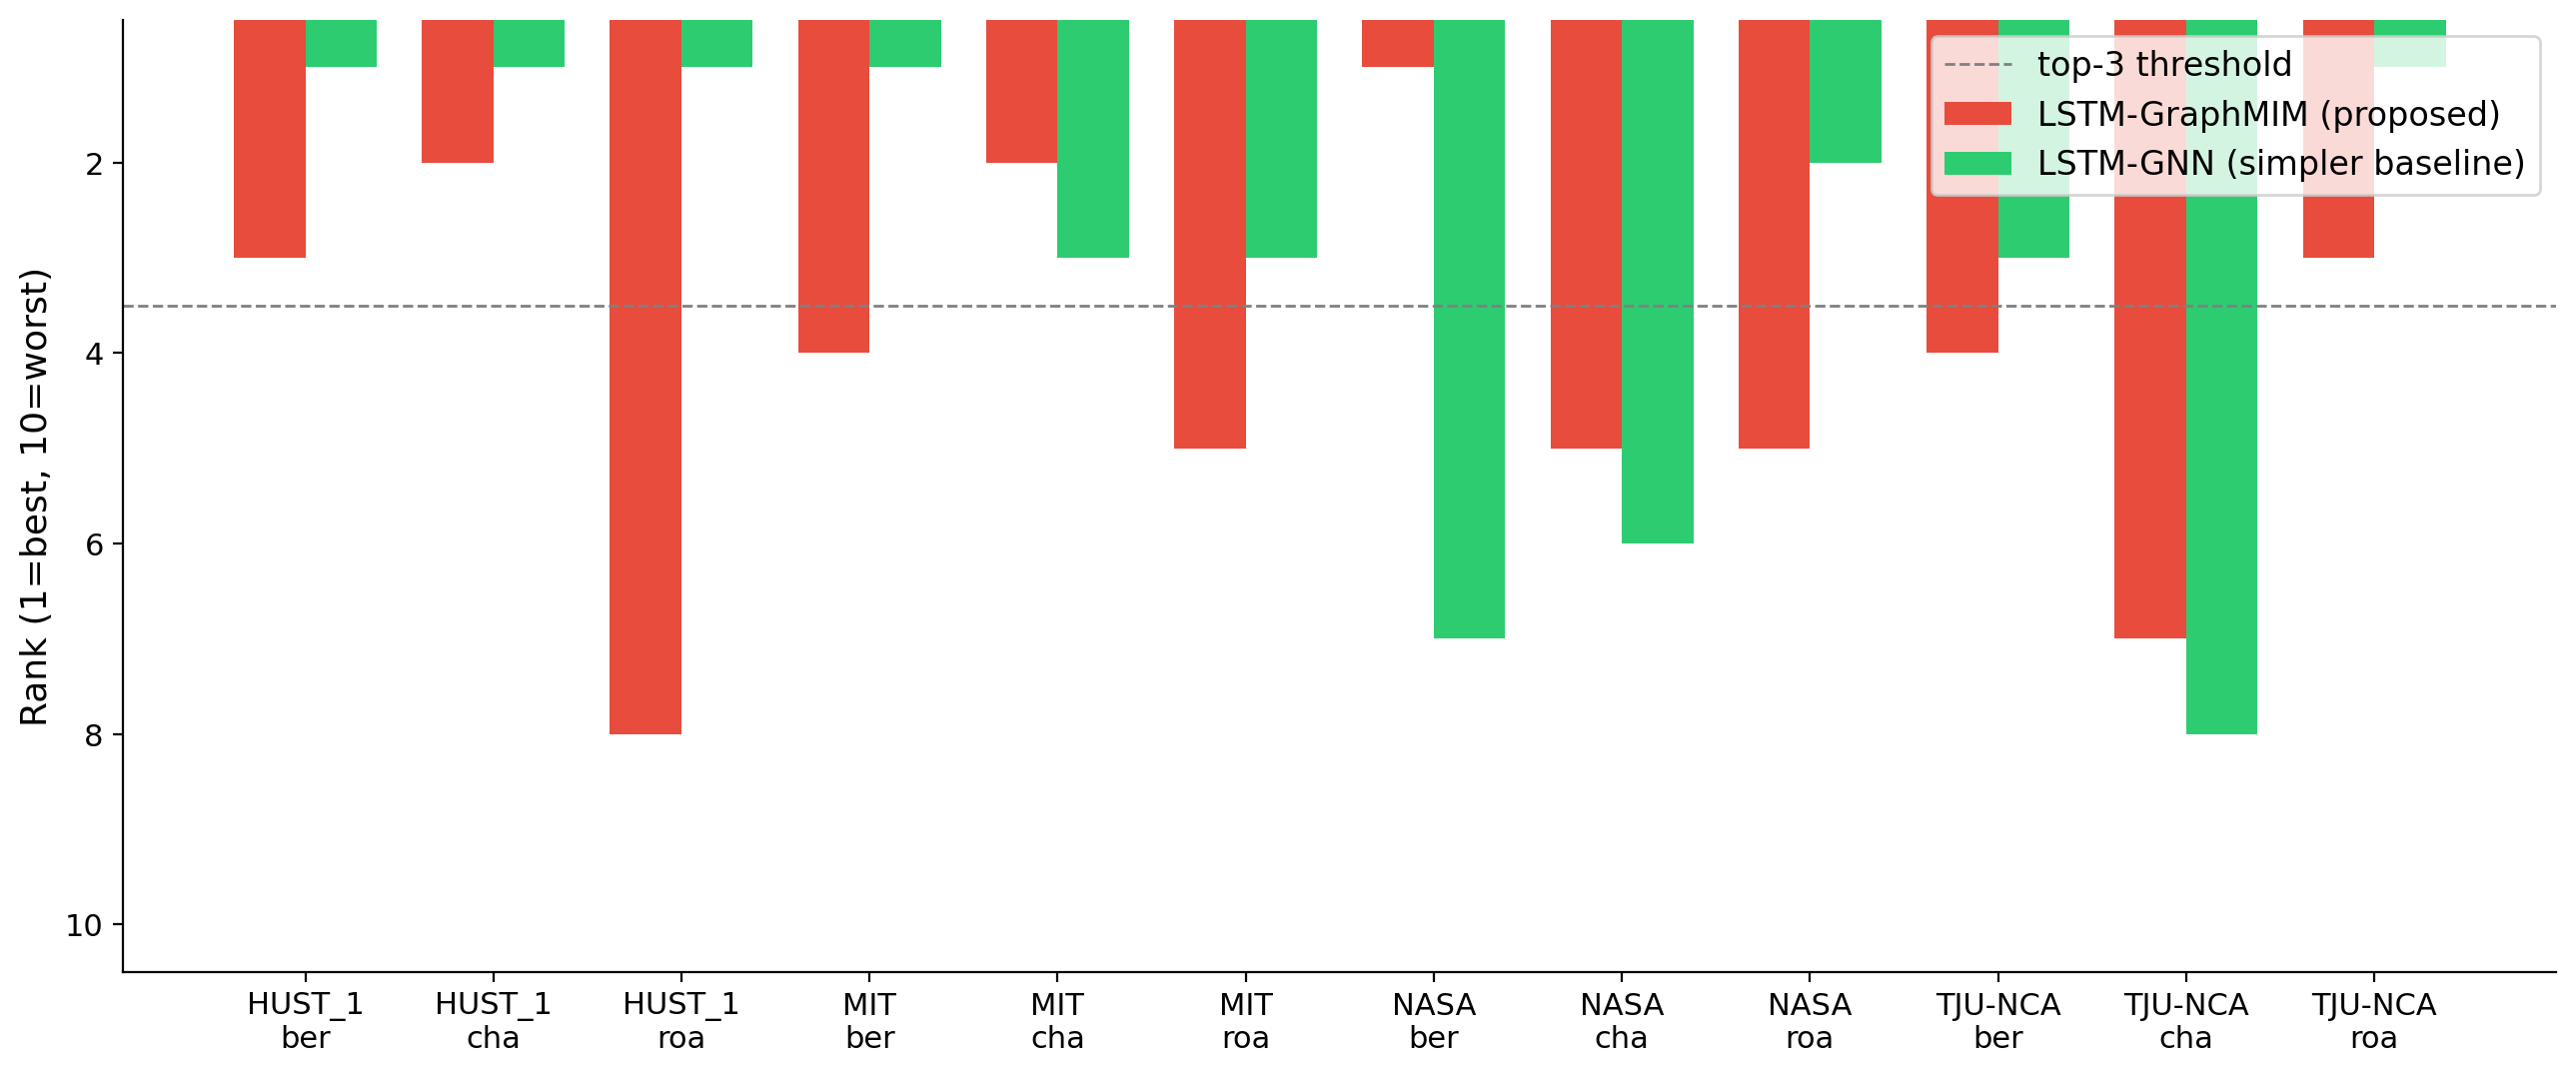
\includegraphics[width=\textwidth]{graphmim_vs_gnn_rank.png}
\end{minipage}\hfill
\begin{minipage}[t]{0.36\textwidth}
\vspace{0em}
\small
\textbf{跨数据集方法总排行（10 方法）}

\vspace{0.5em}
\begin{tabular}{@{}lcc@{}}
\toprule
\textbf{方法} & \textbf{avg rank} & \textbf{top3/12} \\
\midrule
LSTM-GNN       & 3.08 & 9 \\
LSTM-GroupMIM  & 3.33 & 8 \\
LSTM-GraphMIM  & 4.08 & 5 \\
LSTM-MIM       & 4.17 & 6 \\
MLP-GraphMIM   & 6.33 & 2 \\
MLP-MIM        & 6.33 & 2 \\
MLP-GroupMIM   & 6.50 & 2 \\
MLP-GNN        & 7.00 & 2 \\
LSTM-MultiMR   & 7.08 & 0 \\
LSTM-FMG       & 7.08 & 0 \\
\bottomrule
\end{tabular}

\vspace{0.8em}
\textbf{LSTM-GraphMIM：}
\begin{itemize}[leftmargin=1em, itemsep=0pt]
    \item rank=1 次数：1/12
    \item rank$\leq$3 次数：5/12（42\%）
    \item rank$\geq$8 次数：1/12
    \item 排名标准差：2.07
    \item 最好 / 最差：1 / 8
\end{itemize}
\end{minipage}

\footerline
\newpage

%======================================================================
% 封底
%======================================================================
\begin{center}
\vspace*{6cm}
{\Huge\bfseries 报告结束}\\[2em]

\begin{tabular}{@{}rl@{}}
{\large 全部数据可复现，路径见项目 README} \\[0.6em]
{\large 如需查看任意方法 $\times$ 数据集 $\times$ 模式的原始曲线，可另行提供} \\
\end{tabular}
\end{center}

\end{document}
